\documentclass[12pt]{article}
\usepackage{amsmath}
\usepackage{amsfonts}
\usepackage{amssymb}
\usepackage{graphicx}
\graphicspath{{figures/}} % Directory in which figures are stored
\usepackage[natbibapa]{apacite}% \bibliography
\usepackage{float}
\usepackage{hyperref}
\usepackage{amsthm}
\usepackage{xcolor}

\newcommand{\red}{\color{red}}

\title{Statistical methods for microbiome data analysis}
\author{Ka Yat, Liu \\ Supervised by Dr. Jeganathan}
\date{}
\begin{document}
\maketitle
\section*{Abstract}
With the recent innovation of high-throughput sequencing technologies, we can quantify bacteria in different environments much more efficiently. These datasets create demand for researchers to develop various tools to get insights into microbial distribution. In a microbiome data analysis workflow, the raw sequences are denoised to identify the underlying taxonomic groups. Then, after removing DNA contamination, appropriate transformations are used to explore the data. Finally, statistical methods are used for community analyses. This report investigates ways to account for library size differences and Bayesian sampling methods for DNA contamination removal. 

\section{Introduction}
Researchers transform raw sequences to count data for microbial community analyses. However, there are challenges in accounting for the library sizes of different specimens that we should not overlook. The library size is the total count in a specimen.

To account for the difference of library size between specimens, one suggests rarefying the count data by bringing down all samples’ library depth to the same count as the smallest library depth in the data. However, this approach does not account for the heteroskedasticity and raises the variance higher than how the original data describes \citep{mcmurdie2014waste}. Another suggestion is to compute the proportion of each taxon relative to the library size. However, this approach does not consider the uncertainty introduce by the difference in library sizes; hence, it does not consider the effect of heteroskedasticity.

In contrast to treating the DNA sequence as count data, \cite{quinn2018understanding} consider sequencing data as compositional and the data are only meaningful up to the proportions. Specifically, \cite{quinn2018understanding} propose the log-ratio transformation to get insight into community analyses. However, this approach does not account for bias within specimens, i.e., longer genes are more likely to be sequenced \citep{soneson2013comparison}.  

The \texttt{DESeq2} uses the median-of-ratios to compute the library size scaling factor for each sample \citep{anders2010differential} . This method is proportional to the library size but is not skewed by an uncommon high count in one taxon \citep{love2014moderated}.

Researchers have had many successes with DNA sequencing; however, analysis from low-biomass specimens could lead to erroneous results because of DNA contamination \citep{salter2014reagent}. \cite{salter2014reagent} suggest including negative controls to assess the effects of DNA contamination have on the results. \cite{cheng2019combined} propose a Bayesian approach (BARBI) to infer DNA contamination from marker-gene and shot-gun metagenomics data using negative controls. The BARBI uses the posterior density of the true intensity parameter to construct credible intervals. In this study, we approximate the posterior density with grid approximation and use the Markov chain Monte Carlo methods to sample from the posterior density with the provided analytical expression for the density function in the \texttt{BARBI} package. We also discuss a visualization method to  assess the goodness of fit by comparing the data generated from the posterior estimates with the observed counts.

	

\section{Estimating library sizes}

In this report, we use a mock 16S rRNA gene sequencing dataset provided by Zymo Research. The dataset consists of 18 specimens: a known microbial community with seven different levels of dilutions and ten negative controls. We use DADA2 to denoise the raw sequences and assign the taxonomy levels for each amplicon sequence variant (ASV) using a 16S reference database, Silva \citep{callahan2016dada2}. After removing taxa not present in any dilution series specimens, 53 ASVs in the dataset: eight ASVs are related to true species, and the other 45 ASVs are DNA contaminants. We apply rarefaction and DESeq2’s median-of-ratios to estimate the library size effect and compare how each method stabilizes the variance for each ASV after transformation. Assuming that ASV counts are negative binomial random variables, we use inverse hyperbolic sine (arcsinh) transformation to stabilize the variance after removing the library size effect. We also use log-ratio transformation on proportion and visualize the mean-variance relationship. 


\begin{table}[ht]
\caption{Library size of each dilution specimen.}
\centering
\begin{tabular}{l|l|l|l}
  \hline
 Sample ID & Observed & After Rarefied & Median-of-ratios \\ 
  \hline
  Standard.Dilution.1.1 & 12404 & 5183 & 9241\\ 
  Standard.Dilution.1.6 & 21843& 5183 & 41573 \\ 
  Standard.Dilution.1.36 & 14658 & 5183 & 39893 \\ 
  Standard.Dilution.1.216 & 20601 & 5183 & 40705 \\ 
  Standard.Dilution.1.1296 & 18126 & 5183 & 41432 \\ 
  Standard.Dilution.1.7776 & 17779 & 5183 & 20015 \\ 
  Standard.Dilution.1.46656 & 5183 & 5183& 2247\\ 
  Standard.Dilution.1.279936 & 8559& 5183 & 1005 \\ 
   \hline
\end{tabular}
\label{tab:count}
\end{table}

\subsection{Rarefying}

Ecologists introduce rarefying data to compare the richness of species in a community. This method is also used in microbiota analysis because of the common problem where some ASVs counts are relatively lower than other ASVs in the same specimen.

To begin, we propose a minimum value, rarefaction level ,and throw away specimens with counts lower than the minimum. There is no standard formula to calculate the rarefaction level; however, we should keep above 1000 to prevent quality issues. Then, we sample the filtered data without replacement until all specimens have the same count equal to the rarefaction level \citep{navas2013advancing}.

Standard.Dilution.1.46656 from Table \ref{tab:count} has the lowest count of 5183 out of all the specimens, and we, therefore, use it as the rarefaction level. By rarefying the count data, we are adding randomness into our dataset, which would increase proportion variance \citep{mcmurdie2014waste}.

The rarefaction level is crucial when rarefying data. For example, Table \ref{tab:rare_zero} shows one ASV original count in each specimen, arcsinh transformation after accounting for library size differences with rarefying, median-of-ratios, and log-ratio transformation of proportion. We observe that if we decrease the rarefaction level by 86 counts, we would observe an ASV count that transformed from three to zero. In the Zymo data, this ASV appears to be a DNA contaminant, and it does not affect the downstream analysis. However, this could be problematic when computing with low- biomass dataset or rare taxa. 

\begin{table}[ht]
\caption{ASV-49 original count in each specimen, arcsinh transformation after accounting for library size difference with rarefying, median-of-ratios, and log-ratio transformation of proportion.}
\centering
\begin{tabular}{lllll}
  \hline
 Sample ID & Original & Rarefy & Median-of-Ratio & Log ratio \\ 
  \hline
Standard.Dilution.1.1 & 188.00 & 71.00 & 140.09 & 5.24 \\ 
  Standard.Dilution.1.6 & 10.00 & 3.00 & 19.04 & 2.30 \\ 
  Standard.Dilution.1.36 & 225.00 & 76.00 & 612.46 & 5.42 \\ 
  Standard.Dilution.1.216 & 13.00 & 3.00 & 25.66 & 2.56 \\ 
  Standard.Dilution.1.1296 & 9.00 & 2.00 & 20.58 & 2.20 \\ 
  Standard.Dilution.1.7776 & 5.00 & \textbf{0.00} & 5.63 & 1.61 \\ 
  Standard.Dilution.1.46656 & 163.00 & 160.00 & 70.69 & 5.09 \\ 
  Standard.Dilution.1.279936 & 0.00 & 0.00 & 0.00 & -9.21 \\ 
   \hline
\end{tabular}
\label{tab:rare_zero}
\end{table}

\subsection{Median-of-ratios method}

\cite{love2014moderated} implements the median-of-ratios method in \texttt{DESEq2} to estimate the library size scaling factor. To begin, we first compute the geometric mean of each ASV. Then, we calculate the ratio of the count of ASV in each specimen and the geometric mean. Finally, we pick the median-of-ratios as the library size scaling factor. Assuming most of the ASVs are not differentially abundant, the median-of-ratios method will be robust to finding a relevant scaling factor for the library size effects. 

\begin{figure}[H]
	\centering
	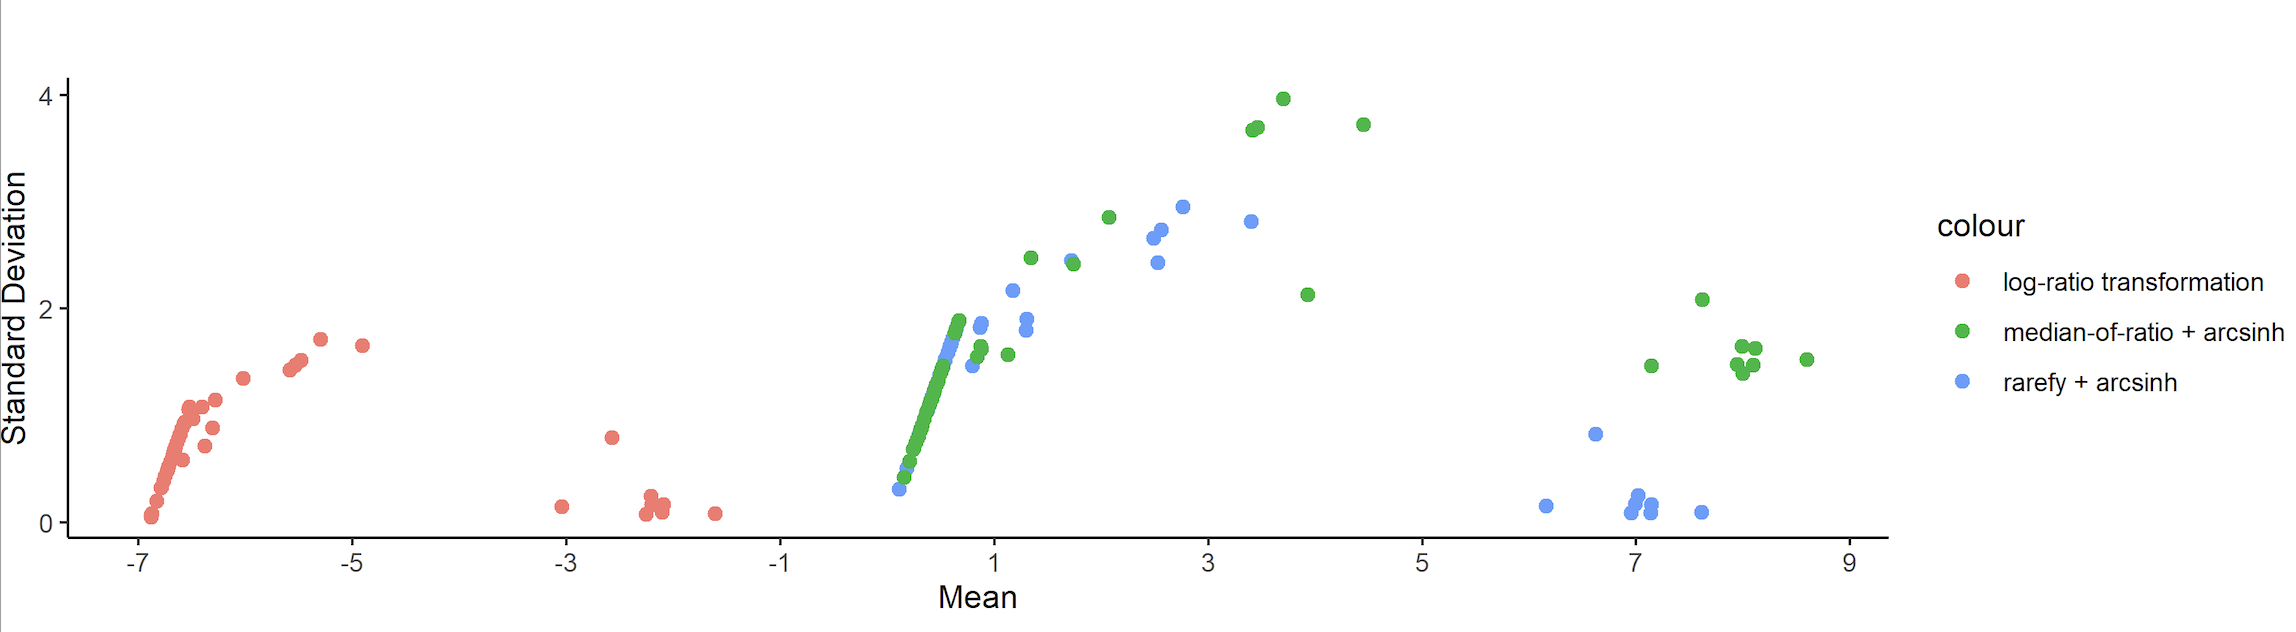
\includegraphics[width=\textwidth]{comparison.png}
	\caption{Comparison of mean-variance of ASVs with three methods for accounting library size differences: median-of-ratios, rarefying, proportion.}
	\label{fig:lib}
\end{figure}


Figure \ref{fig:lib} shows the standard deviation versus mean for each ASV with three methods for accounting library size differences: median-of-ratios, rarefying, proportion. We observe similar patterns in mean-variance dependence for all three transformations, but the range of values varies. The median-of-ratios method with arcsinh transformation has the largest range of mean, whereas the other two methods have a similar range. A slight linear pattern is observed for the smaller mean values in all three methods. Lastly, eight ASVs are identified in a similar position to the right of the points in all three methods. Seven of the eight ASVs are associated with the true species in the mock data, and the other ASV is a DNA contaminant. 


\section{Density approximation and samplers}

The BARBI workflow uses median-of-ratios to compute library size scaling factors.  Then, the BARBI method involves sampling from a posterior density with a one-dimensional sample space. Here we explore grid approximation to approximate the posterior density, Monte Carlo methods, and Markov chain Monte Carlo (MCMC) to draw samples from the posterior density derived in the BARBI method. 

\newtheorem{definition}{Definition}
\begin{definition}
Given a random variable $X$, the density $f_X(x)$ is a probability density function, if:
\begin{enumerate}
	\item {$f_X(x) \geq 0 , \forall x \in \chi,$}
	\item {$\int_{\chi}f_X(x) dx  = 1, $}
	\item {$ P( x \in A ) = \int_{x \in A} f_X(x) dx$, where $\chi$ is the support of X and  $A \subset \chi.$}
\end{enumerate}
\end{definition}

\subsection{Grid Approximation}

We use grid approximation to approximate a density function. First, we propose a discrete interval (grid) with all possible $x$ values that cover the sample space of $X$. Then, we approximate the posterior density function by evaluating the density at each value on the grid. Figure \ref{fig:ga} shows the results of grid approximation for four ASVs in the non-diluted specimen in the Zymo data.


\begin{figure}[H]
	\centering
	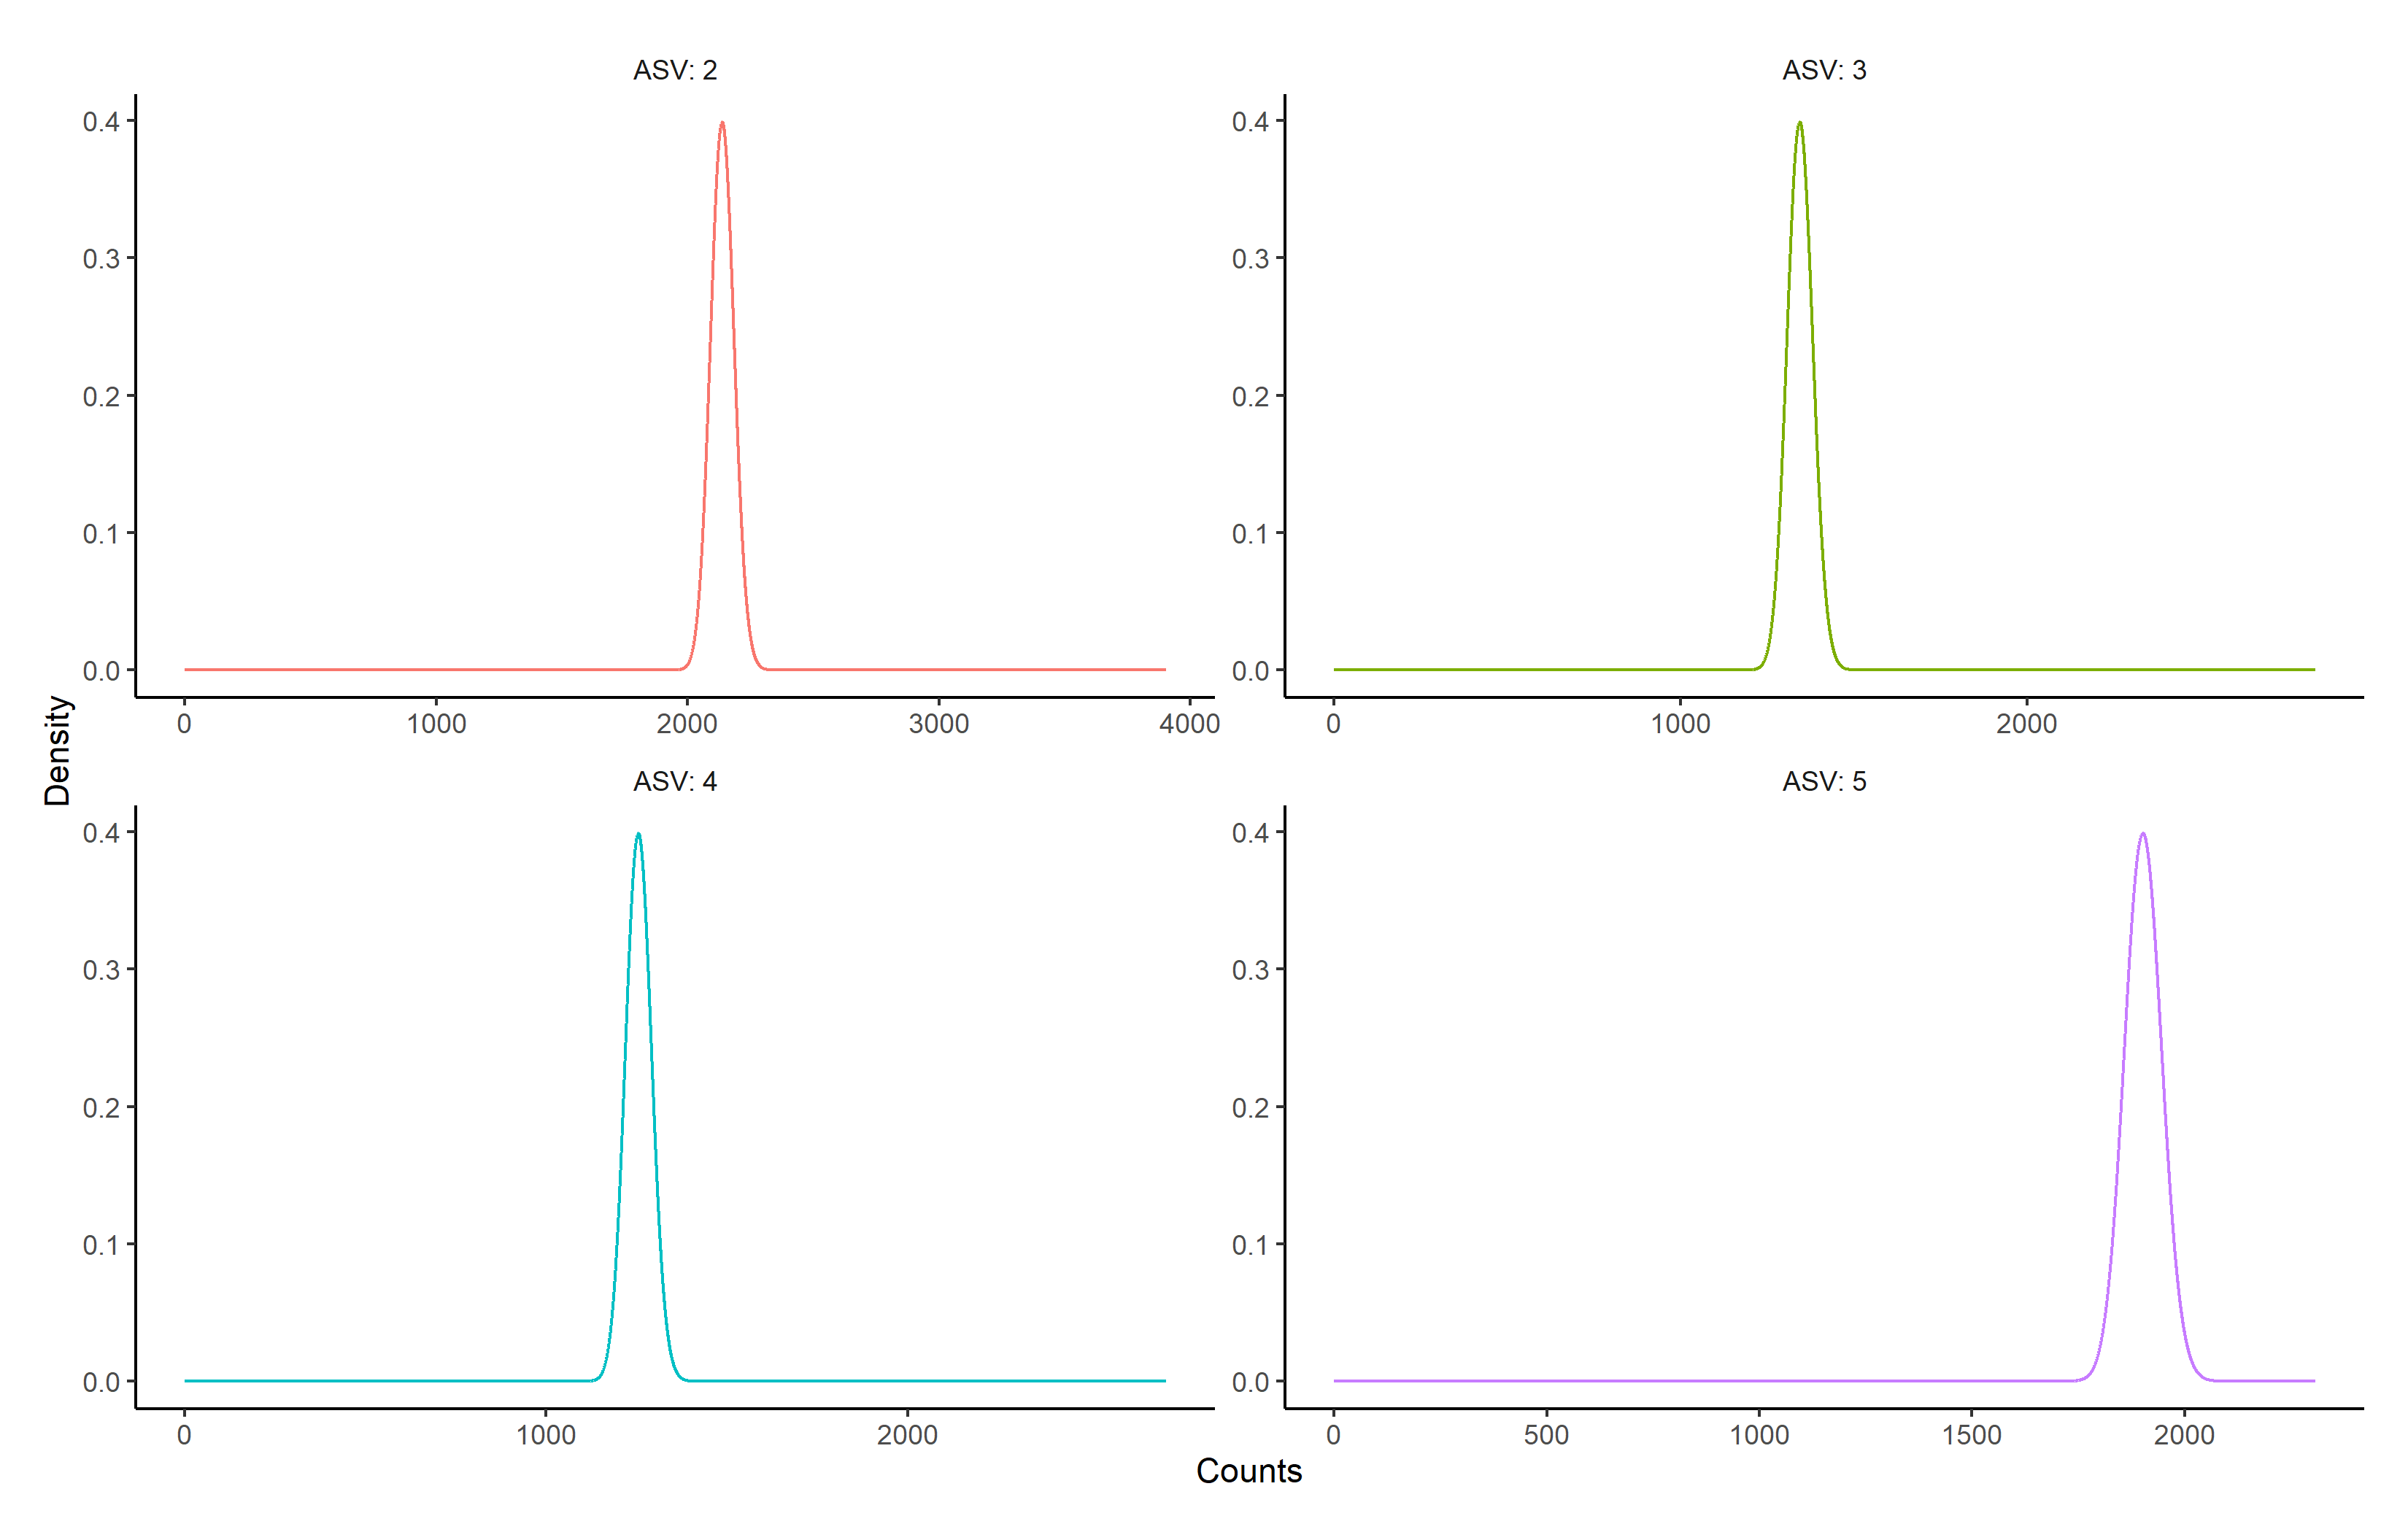
\includegraphics[width=\textwidth]{ga_sample.png}
	\caption{Grid approximation of the posterior density for four ASVs in the non-diluted specimen in the Zymo data.}
	\label{fig:ga}     
\end{figure}

\subsubsection{Challenges}

The choice of the grid is crucial for grid approximation, as the compactness of the grid affects the completeness of the approximation. The closer two adjacent values are in the grid, the more points the algorithm needs to compute for the same interval. As a result, we get a more detailed approximation with a tighter grid. However, since we compute every value in the grid, the method becomes more computationally expensive as we increase the number of points. In particular, grid approximation suffers from the curse of dimensionality. 

\subsection{Rejection Sampling}

Rejection Sampling is a Monte Carlo method that samples from the density function (Wells, Casella, and Robert (2004)). It requires us to explicitly know the density function, which we call the target density $f(x)$. Next, we suggest a proposal density that covers the same sample space as the target density. Then, we scale the proposal density by a constant $C$, such that the proposal density completely encloses the target. Finally, we independently sample from the proposal density, and the sample will be accepted with a probability of $\dfrac{f\left(x\right) }{Cg\left(x\right)}$. The sampling is repeated until we are satisfied with the number of samples. We use the package \texttt{AR} in R to perform rejection sampling. Then, we use \texttt{ggplot2} to visualize the histogram of posterior samples. Figure \ref{fig:rs} shows the histograms of posterior samples using rejection sampling of four ASVs in the non-diluted specimen in the Zymo data.

\begin{figure}[H]
	\centering
	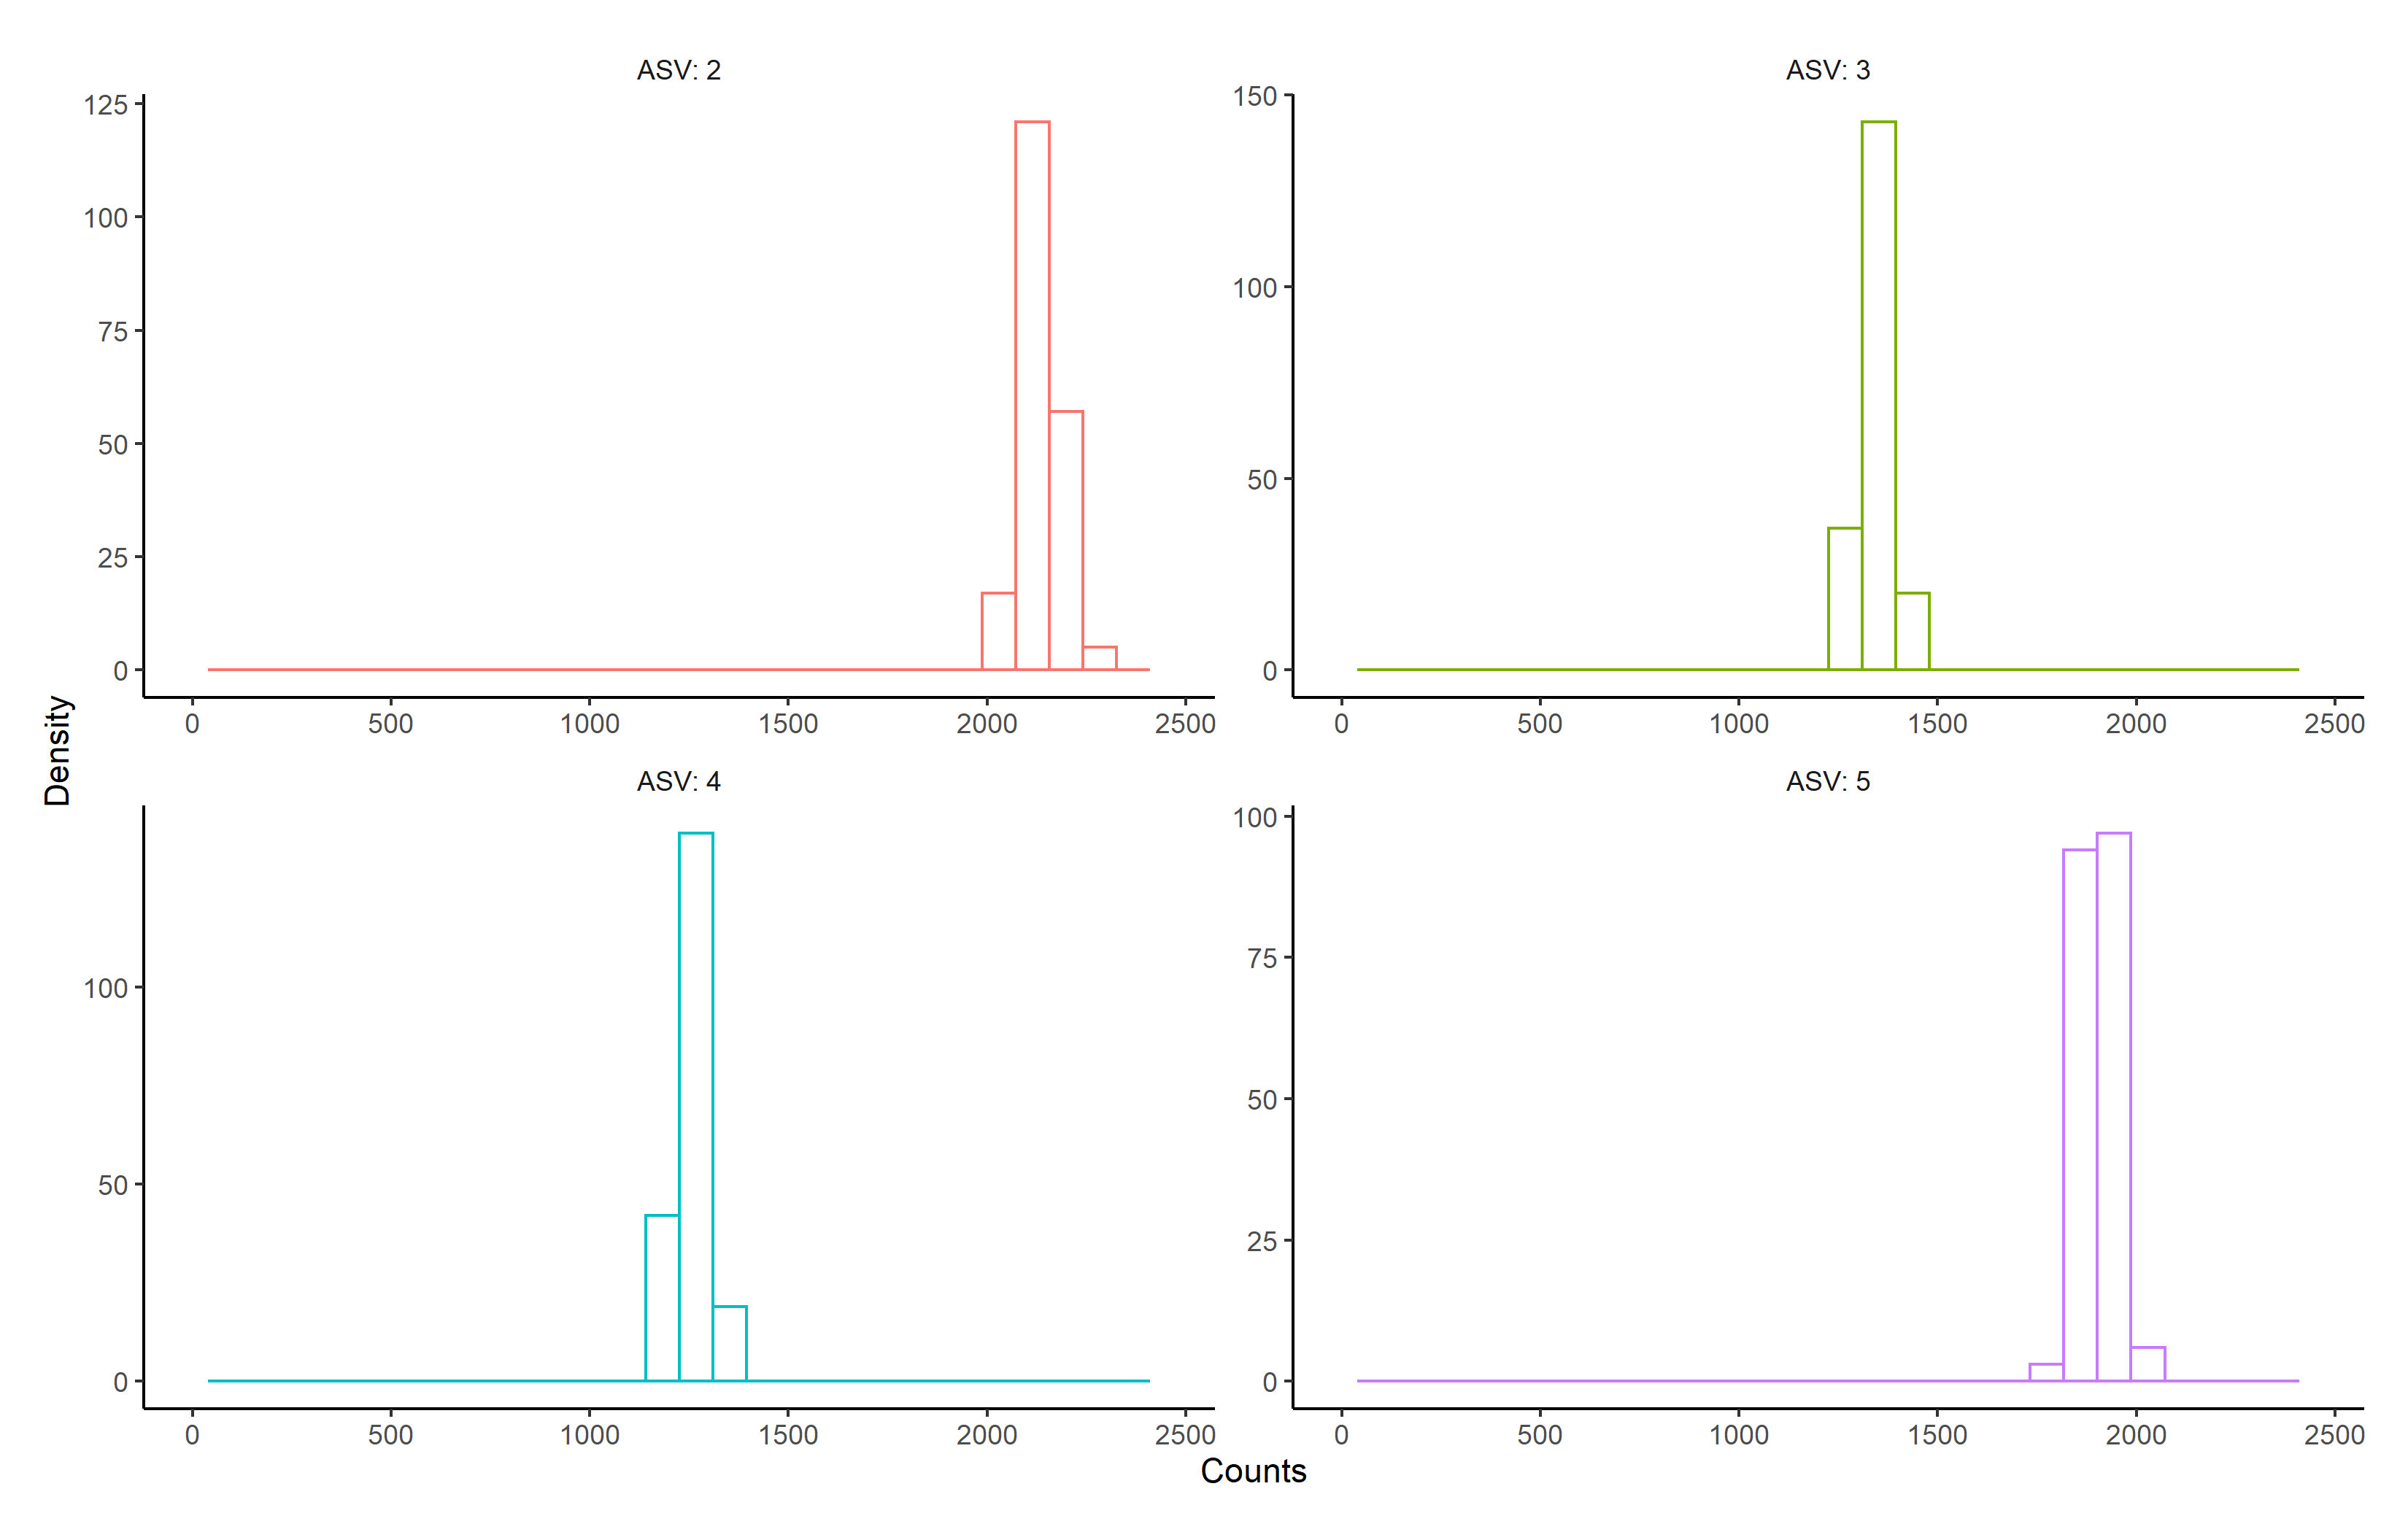
\includegraphics[width=\textwidth]{rejection_sampling.png}
	\caption{Histogram of posterior samples using rejection sampling for four ASVs in the non-diluted specimen in the Zymo data.}
	\label{fig:rs}     
\end{figure}

\subsubsection{Challenges}
The choice of proposal density is crucial. We should aim to find a proposal density sample space as close as possible to the target density, such that we do not cover out of sample space. We generally want a lower constant $C$ and a low rejection ratio for more efficiency. The rejection sampling also suffers from the curse of dimensionality. Moreover, the rejection sampling method requires that the probability density of the target is known to compute the acceptance ratio. This could be problematic if we want to sample from a density up to a constant. In Bayesian inference for high-dimensional sample space, the posterior density is often known up to a constant, so rejection sampling is not helpful for this case. For high-dimensional sample space, Markov chain Monte Carlo can be considered. 

\subsection{Metropolis–Hastings Algorithm}

The Metropolis-Hasting algorithm is a Markov chain Monte Carlo method \citep{hastings1970monte}. In this sampler, the samples draws from the posterior density are not independent compared to rejection sampling. The Metropolis-Hasting algorithm is as follows.

\textbf{Steps:} For any probability density $f(x)$, we need a proposal density $q(x)$ proportional to $f(x)$ and that the density function of $q(x)$ is known. However, the density function of the target can be known up to a constant. 

\begin{enumerate}
	\item Identify $x_0$ as an initial value.
	\item {Calculate the acceptance ratio $\alpha= \text{min}\left(\frac{f(x_{t})}{f(x_{t-1})}\times\frac{q(x_{t-1}|x_{t})}{q(x_{t}|x_{t-1})}, 1\right)$, where $t$ is the $t^{\text{th}}$ draw}
	\item {Generate a random number, $u_t$ from $U \sim \text{Uniform}(0,1)$}.
	\begin{enumerate}
		\item {Accept $x_t$ if $\alpha > u_t$}.
		\item {Reject $x_t$ and replace with $x_{t-1}$ if $\alpha \leq u_t$}.
	\end{enumerate}
\end{enumerate}


Figure \ref{fig:mh} shows the histograms of posterior samples using the Metropolis-Hasting algorithm for four ASVs in the non-diluted specimen in the Zymo data.
We use the \texttt{MH\_MCMC}, in the \texttt{BARBI} package to sample from the posterior density.

\begin{figure}[H]
	\centering
	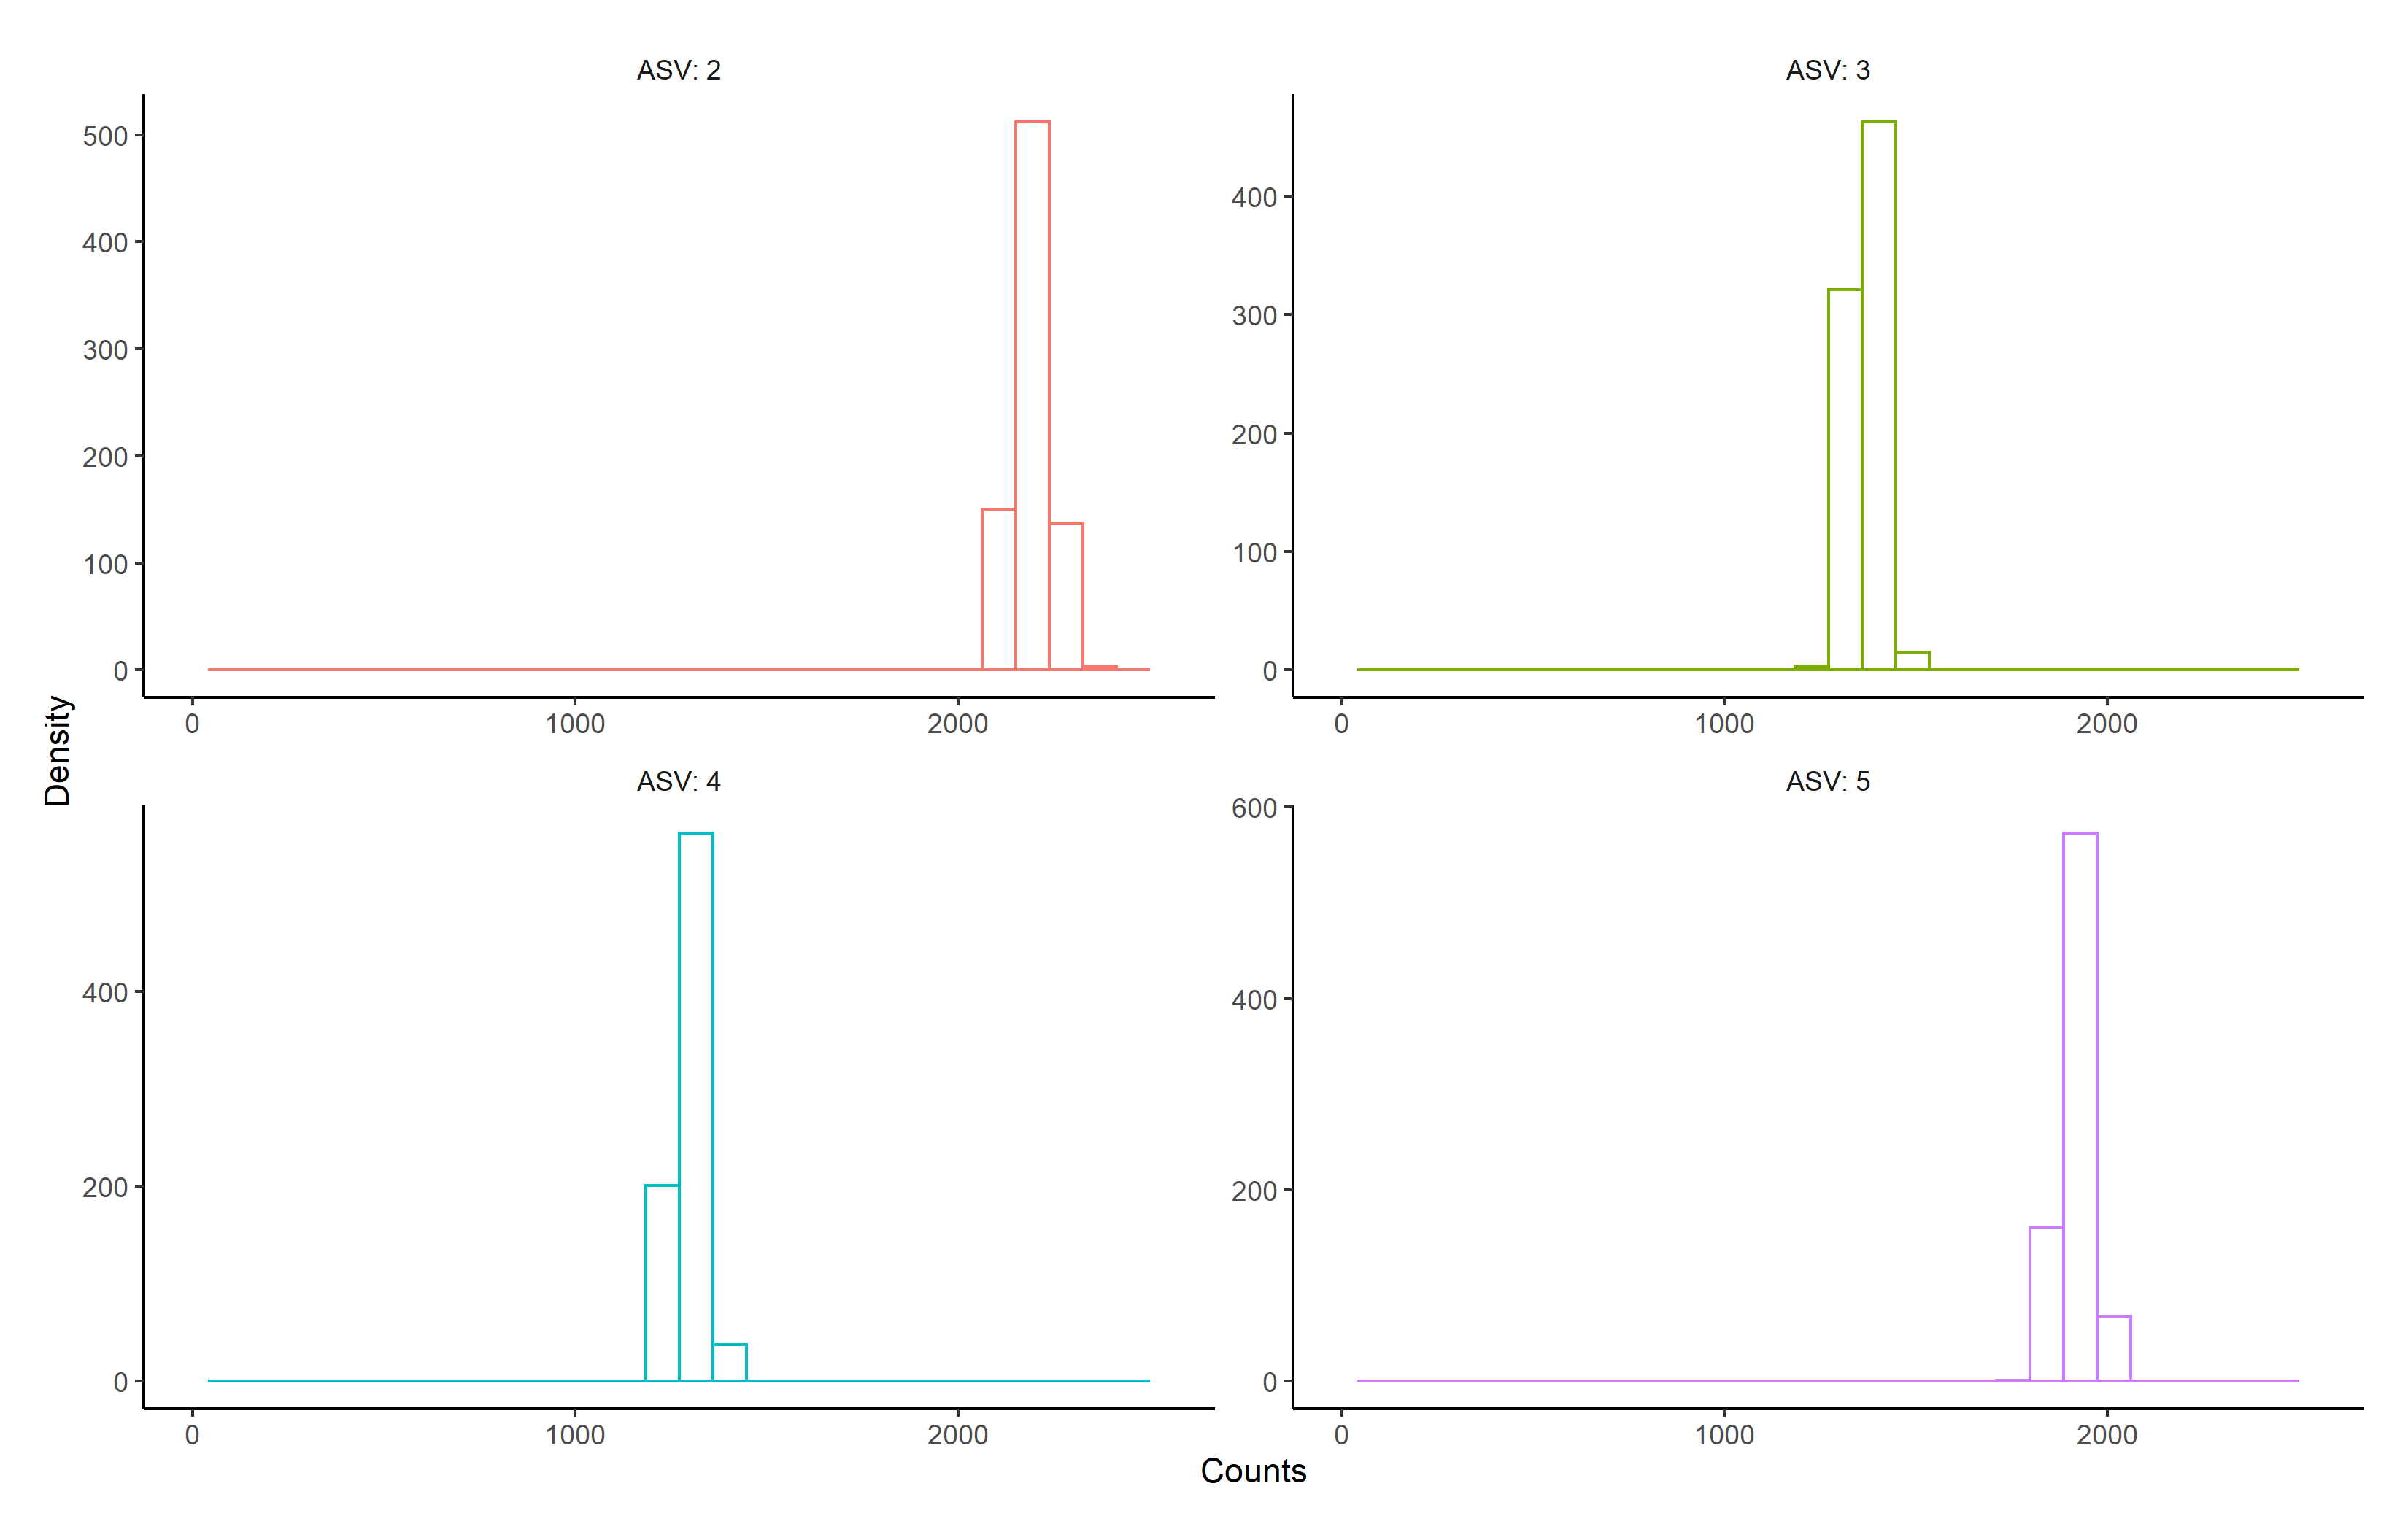
\includegraphics[width=\textwidth]{metropolis_hasting.png}
	\caption{Histogram of posterior samples using Metropolis-Hasting for four ASVs in the non-diluted specimen in the Zymo data.}
	\label{fig:mh}     
\end{figure}

\subsubsection{Challenges}
Though the Markov property improves the efficiency of the sampling, but could also be challenging. MCMC methods come with the cost of non-independent samples. We can detect this problem using the trace plot as in Figure \ref{fig:trace} for one ASV. MCMC, in general, suffers from autocorrelation. Different adjustments can be made to tackle this problem. One approach is through ”thinning,”  which only keeps every $n^{\text{th}}$ sample of the chain \citep{link2012thinning}.  

If the starting value of Metropolis-Hasting is far from the sample space, it will take numerous steps before reaching the target density because of the Markov property. Hence, the starting value of Metropolis-Hasting is critical.  One approach to handling this problem is to discard the initial samples, also known as the burn-in period (\cite{gelman1995bayesian}). Figure \ref{fig:trace} shows that with a starting value of 0, the samples from the early iterations do not follow the target density. The dashed line represents the 0.1st and 99.9th percentile. The two samples outside the interval are from the initial 50 iterations. Therefore, we discard the first 50 iterations as the burn-in period. 

\begin{figure}[H]
	\centering
	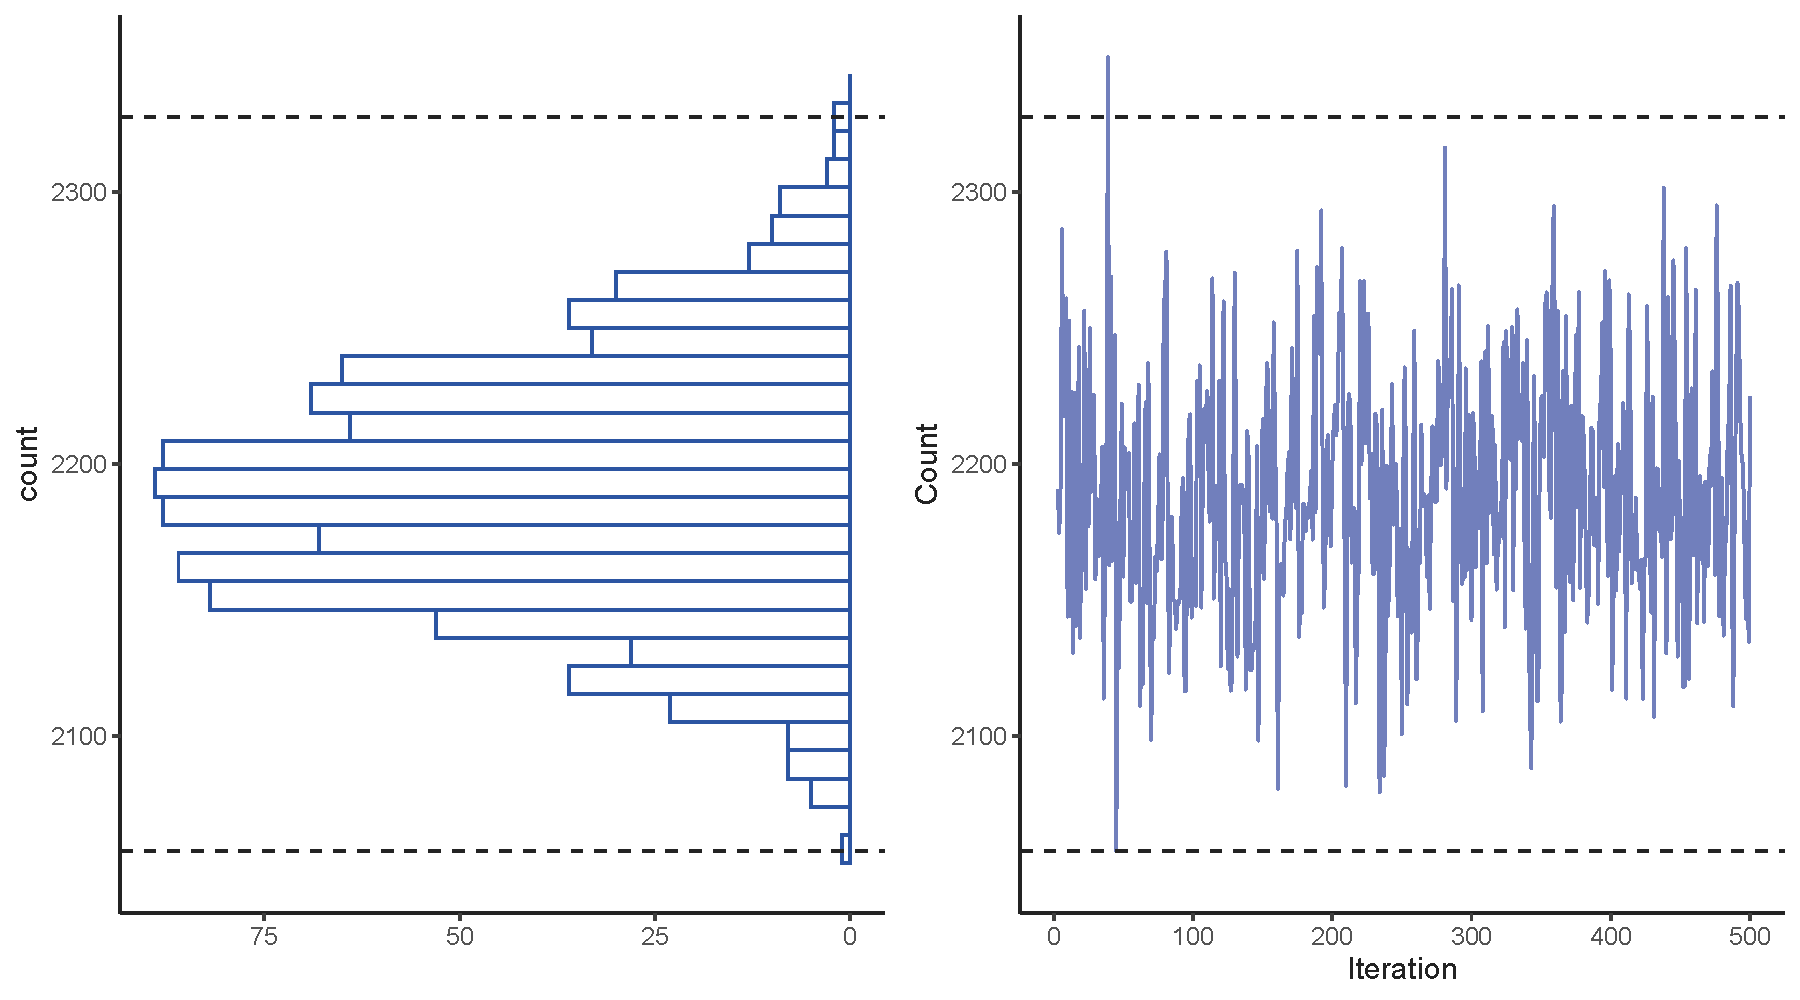
\includegraphics[width=\textwidth]{hist_trace.png}
	\caption{Histogram(sample space on the vertical axis) and trace plot of applying Metropolis-Hasting algorithm to ASV 2 in the non-diluted specimen with a starting value of 0.}
	\label{fig:trace}     
\end{figure}

\subsection{Goodness of fit}

We access the goodness of fit for the BARBI method by comparing the data generated from the posterior estimate with the observed counts. First, we use the posterior estimates of the model parameter using the rejection sampling and generate ASV counts from the known hierarchical mixture model. Then, we make a histogram of the generated counts and present the observed count as a vertical line on the histogram. We expect the vertical line lies within the support of the histogram. Figure \ref{fig:good_rs} shows that the BARBI method has a good fit because all four observed counts are positioned near the mode of the predicted density.

\begin{figure}[H]
	\centering
	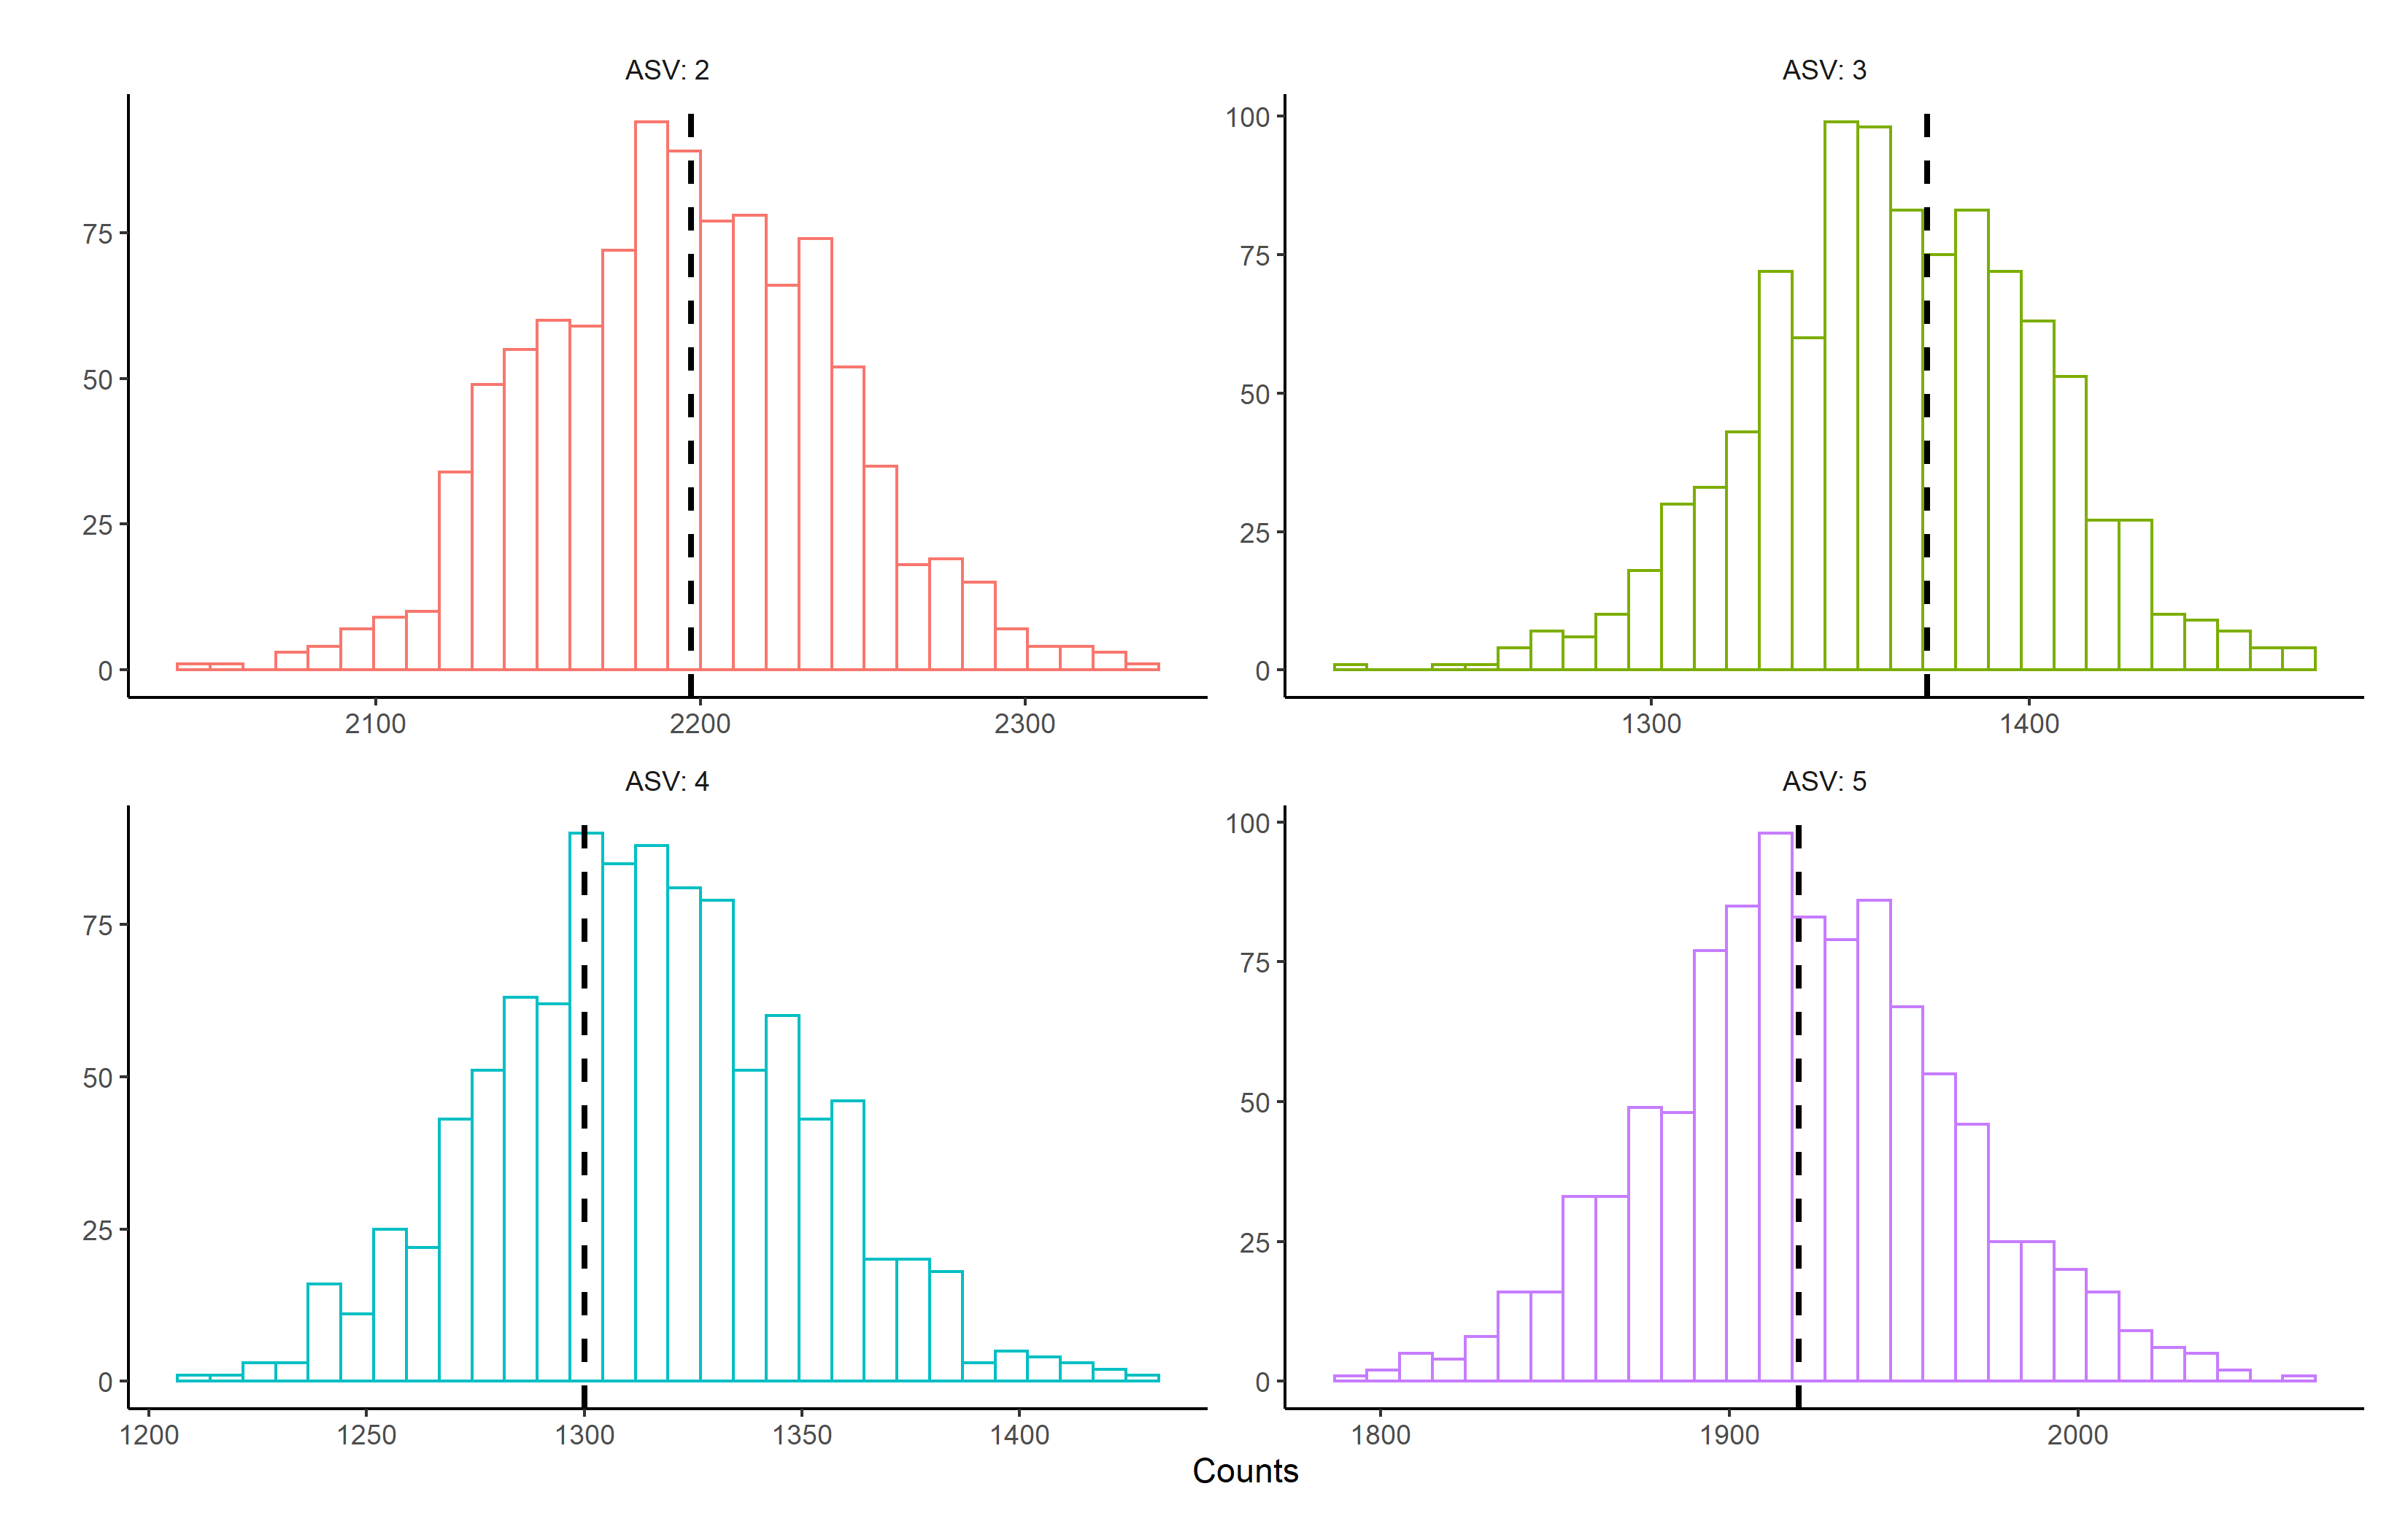
\includegraphics[width=\textwidth]{goodness_rs.png}
	\caption{Goodness of fit for the BARBI method by comparing data generated from the posterior estimates using rejection sampling with the observed counts (vertical line).}
	\label{fig:good_rs}     
\end{figure}


We also access the goodness of fit of the BARBI method when we use Metropolis- Hasting algorithm. In figure \ref{fig:good_mh}, all four plots show evidence that the observed counts of the ASVs lie within the support of the histogram. 


\begin{figure}[H]
	\centering
	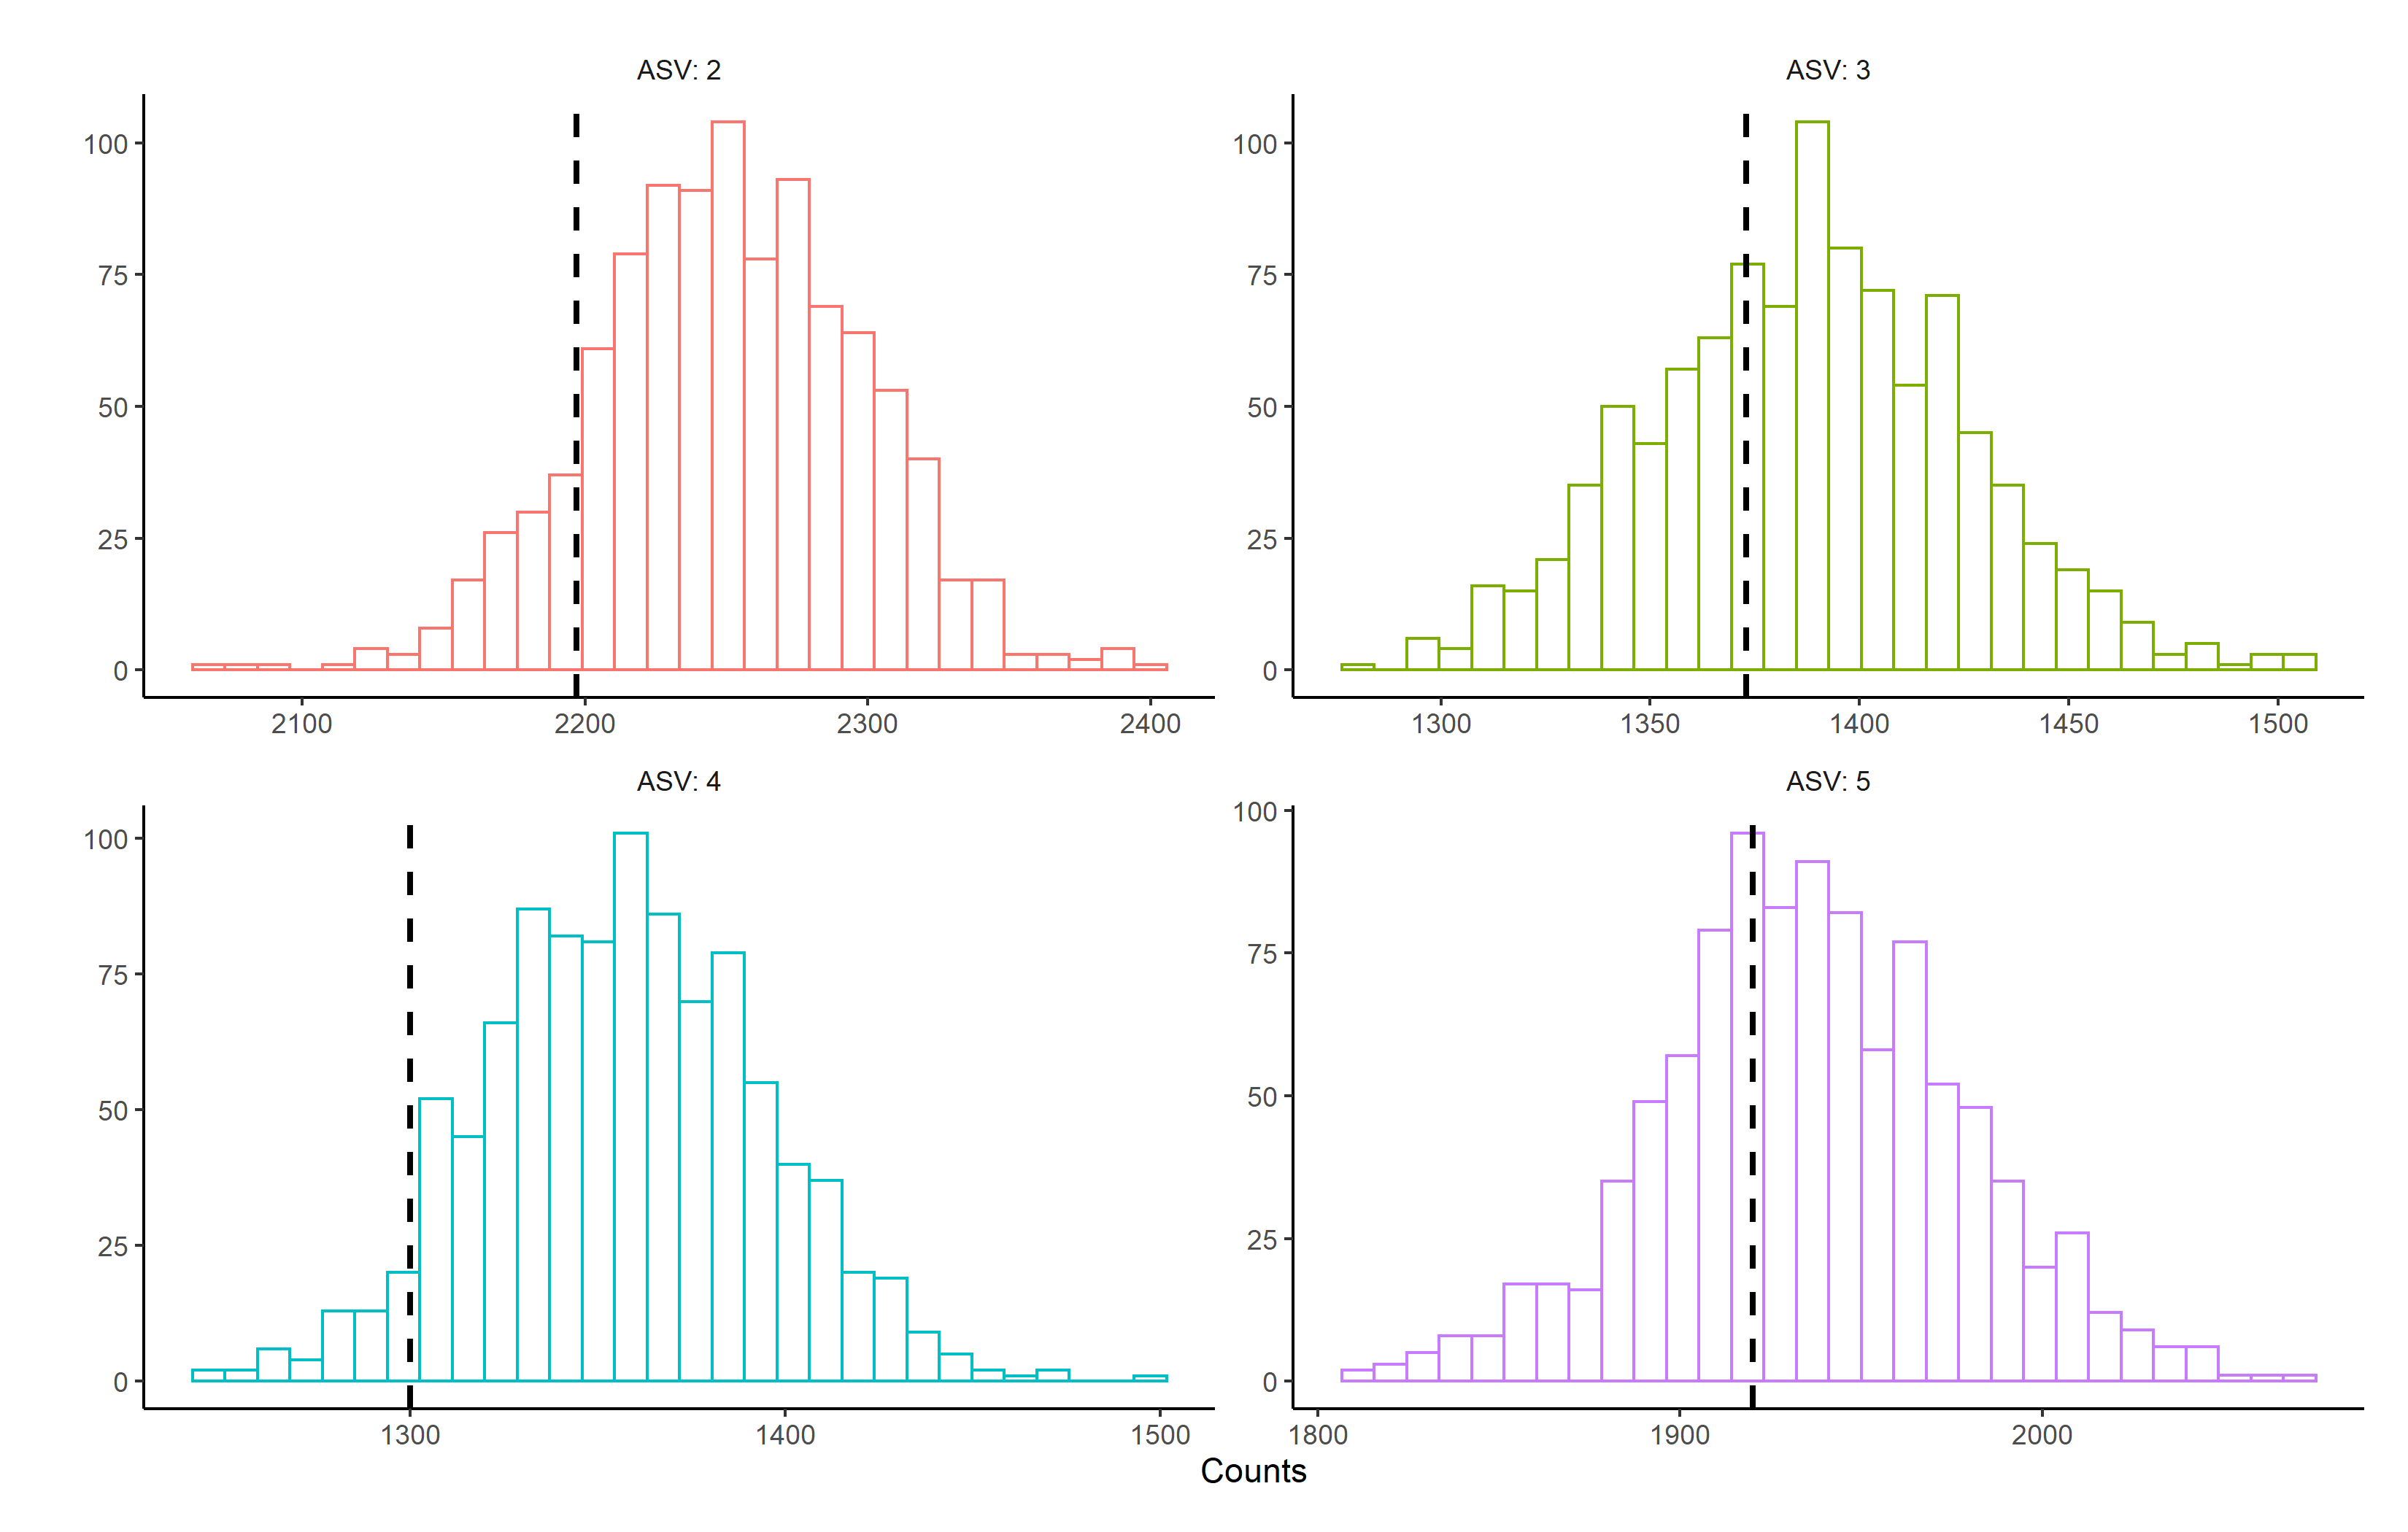
\includegraphics[width=\textwidth]{goodness_mh.png}
	\caption{Goodness of fit for the BARBI method by comparing data generated from the posterior estimates using Metropolis-Hasting with the observed counts (vertical line).}
	\label{fig:good_mh}     
\end{figure}



\section{Discussion}

High-throughput sequencing technology provides researchers efficient ways to quantify bacteria. DNA strands are broken down into fragments of sequences for community analyses. However, there are many debates and methods on how to retrieve the information. In this report, we discussed the rarefying, median-of-ratios, and proportions methods for accounting for library size differences. We found that low counts ASVs are sometimes identified as zero counts with the rarefying, which is challenging, especially for rare taxa and low-biomass data. 

DNA contamination is a big challenge for low-biomass data. The BARBI method can identify and remove DNA contamination from low-biomass data. This workflow uses the analytical expression for the posterior density of a one-dimensional sample space. We use this posterior density to explore gird approximation and different sampling methods, such as rejection sampling and the Metropolis-Hasting algorithm. We found that choosing an appropriate burn-in period provides a solution with a random starting value. Finally, we discuss a visualization method to do goodness of fit for the BARBI method which can be extended to different applications. 

\section{Accomplishments}

During the summer research period, I learned the data analysis with micro- biome data from the beginning. We prepared a research schedule that included readings on count data modeling, high throughput sequencing data, 16s rRNA gene sequencing data, Bayesian statistics, and computation. Through the readings, I learned about the challenges in molecular microbial data analysis, such as library size differences and DNA contamination. 

I have had extensive uses of R, LATEX, Github, Overleaf, and running inline codes to high-performance computing throughout the research. 
In addition, I had the opportunity to network from the conferences and group meetings. For example, at the Bioconductor conference, I learned about cutting-edge researches on microbiome data analysis. In the weekly group meetings, I had built relationships with students from very different fields. 

\newpage
\bibliographystyle{apacite}
\bibliography{KaYat_StewartResearch_Report}

\end{document}